\documentclass[10pt,a4paper]{report}
%\usepackage[latin1]{inputenc}
\usepackage[utf8]{inputenc}
\usepackage{amsmath}
\usepackage{amsfonts}
\usepackage{amssymb}
\usepackage{graphicx}
\usepackage{multicol}
\usepackage{tabularx}
\usepackage{tikz}
\usetikzlibrary{arrows,shapes,automata,petri,positioning,calc}
\usepackage{hyperref}
\usepackage{tikz}
\usetikzlibrary{matrix,calc}
\usepackage[margin=0.5in]{geometry}
\newenvironment{Figure}
  {\par\medskip\noindent\minipage{\linewidth}}
  {\endminipage\par\medskip}
\begin{document}
%--------------------logo figure-------------------------%
\begin{figure*}[!tbp]
  \centering
  \begin{minipage}[b]{0.4\textwidth}
    
\includegraphics[scale = 0.05]{iitlogo.jpg}
  \end{minipage}
  \hfill
  \vspace{5mm}\begin{minipage}[b]{0.4\textwidth}
\raggedleft  
\includegraphics[scale = 0.10]{nrc.png}\

  \end{minipage}\vspace{0.2cm}
\end{figure*}
%--------------------name & rollno-----------------------
\raggedright \textbf{Name}:\hspace{1mm} Chirag Shah\hspace{3cm} \Large \textbf{Assignment-4}\hspace{2.5cm} % 
\normalsize \textbf{Roll No.} :\hspace{1mm} FWC22053\vspace{1cm}
\begin{multicols}{2}

\textbf{Triangle Law of Vector addition }
\vspace{0.5cm}\raggedright \\
The triangle law of vector addition says that when two vectors are represented as two sides of a triangle with the same order of magnitude and direction, then the magnitude and direction of the resultant vector is represented by the third side of the triangle taken in reverse order..\vspace{3mm} \\ 
\begin{equation}
\boldsymbol{R}=\boldsymbol{A}+\boldsymbol{B} 
\end{equation}
%------------------------trifig-------------------%
\vspace{2mm}\textbf{Vector addition }
 \begin{center}
 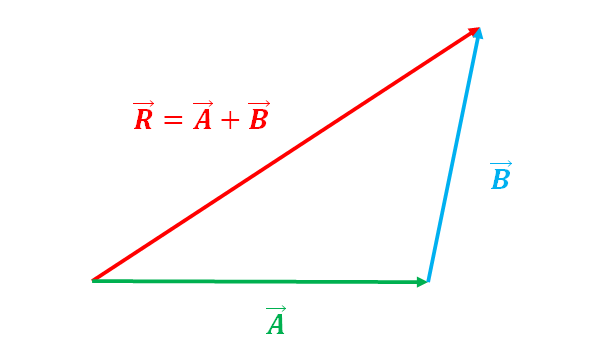
\includegraphics[width=0.5\textwidth]{tri.png}  
 fig 1.1   \vspace{2mm}\\
 \end{center}\vspace{5mm}
%------------------------working-------------------%
\textbf{Dot product}\vspace{1mm}
\raggedright \\When two vectors a and b are perpendicular then their dot product is 0:\vspace{3mm} 
\begin{equation}
\boldsymbol{a}.\boldsymbol{b}=\boldsymbol{||a||}\hspace{0.5mm}\boldsymbol{||b||}cos(\theta)
\end{equation}
\vspace{2mm}
\raggedright And since they are perpendicular then the angle between them is 90.\\
\vspace{2mm}
\begin{equation}
\boldsymbol{a}.\boldsymbol{b}=\boldsymbol{||a||}\hspace{0.5mm}\boldsymbol{||b||}cos(90^{\circ})=0
\end{equation}
%----------------problem statement--------------%
\raggedright \textbf{Problem Statement:}\vspace{2mm}
\raggedright \\Construct a right triangle whose base is 12cm and sum of its hypotenuse and other side is 18cm.
\vspace{5mm}

%-----------------------------solution---------------------------
\raggedright \textbf{SOLUTION}:\vspace{2mm}\\
Let A,B and C be the vertices of right triangle with with coordinates (0,0), (12,0) and (0,k) respectively.\vspace{2mm}\\
OB-Base.
AB-Hypotenuse.
OA-Side.\\\vspace{2mm}
%---------given----------------%
\raggedright \textbf{Given}:\vspace{2mm}\\
Since its a right triangle OA $\perp$ OB \\\vspace{2mm}
Since base is 12cm length of OB = 12  \\i.e,\\
\begin{equation}
\boldsymbol{||b||}= 12 \vspace{2mm}
\end{equation}
Sum of length OA and AB = 18cm \\ i.e,\\
\begin{equation}
\boldsymbol{||a||} + \boldsymbol{||c||}= 18 \vspace{2mm}
\end{equation}
%-------------To find ------------------%
\textbf{To Find}\vspace{2mm}\\
The magnitude of $\boldsymbol{a} i.e  \boldsymbol{||a||}$\\\vspace{2mm}
%--------------steps----------------------%
\textbf{STEP-1}\vspace{2mm}\\
Let k be the unknown point in the vertex A \vspace{2mm}\\
Then coordinates of vertices  O,A and B are :\vspace{2mm}\\
 O(0,0)\vspace{1mm} \\ B(12,0)\vspace{1mm} \\A(0,k)\vspace{1mm} \\
\vspace{3mm} 
We know that $\boldsymbol{||a||} + \boldsymbol{||c||}= 18 $\vspace{2mm}\\
So, Let x=18 
\begin{equation}
    \boldsymbol{||a||} + \boldsymbol{||c||}= x \vspace{2mm}
\end{equation}
We know that , \\
\begin{equation}
    \boldsymbol{||c^2||} = \boldsymbol{||a^2||} + \boldsymbol{||b^2||} \vspace{2mm}
\end{equation}

Since OA $\perp$ OB  i.e $\boldsymbol{a}$ $\perp$  $\boldsymbol{b}$ \\\vspace{3mm}
From Dot product \\
\begin{equation}
\boldsymbol{a}.\boldsymbol{b} = 0 
\end{equation}\vspace{2mm}\\

\textbf{STEP-2}\vspace{2mm}\\
(1.) If we find $\boldsymbol{||a||}$  we can get k in A(0,k) \\\vspace{2mm}
\begin{equation}
    O=\begin{pmatrix}
0\\
0
\end{pmatrix} 
    B=\begin{pmatrix}
12\\
0
\end{pmatrix} 
    A=\begin{pmatrix}
0\\
k
 \end{pmatrix}  \vspace{3mm}
\end{equation}
  
By using equation (7)
\begin{center}
    $ \boldsymbol{||c^2||} = \boldsymbol{||a^2||} + \boldsymbol{||b^2||}$ \vspace{2mm}
\end{center}
\begin{equation}
    \boldsymbol{||b^2||} = \boldsymbol{||c^2||} - \boldsymbol{||a^2||} \vspace{2mm}
\end{equation}
We know that $\boldsymbol{||c^2||} - \boldsymbol{||a^2||} =  \boldsymbol{||c-a||*||c+a||}$\vspace{2mm}\\
Since, $ \boldsymbol{||c+a||}=x$
\begin{equation}
    \boldsymbol{||b^2||} = \boldsymbol{||c-a||}*(x) \vspace{2mm}
\end{equation}
\begin{equation}
  \boldsymbol{||c-a||} = \frac{ \boldsymbol{||b^2||}}{x}
\end{equation}
And ,
\begin{equation}
    \boldsymbol{||c+a||} = x \vspace{2mm}
\end{equation}
Using equation (12) and (13),
\begin{equation}
  \begin{pmatrix}
1 & 1\\
1 &-1
\end{pmatrix} 
\begin{pmatrix}
c\\
a
\end{pmatrix} = \begin{pmatrix}
x\\
\frac{ \boldsymbol{||b^2||}}{x}
\end{pmatrix} 
\end{equation}\vspace{2mm}\\

\textbf{STEP-2}\vspace{2mm}\\
Using equation (14) \vspace{2mm}\\
 Let,
\begin{equation}
  P =\begin{pmatrix}
1 & 1\\
1 &-1
\end{pmatrix} 
\end{equation} \\ \vspace{2mm}
\begin{equation}
  y =\begin{pmatrix}
c \\
a
\end{pmatrix} 
\end{equation}  \vspace{2mm}

\begin{equation}
  Q = \begin{pmatrix}
x\\
\frac{ \boldsymbol{||b^2||}}{x}
\end{pmatrix} 
\end{equation}\vspace{2mm}
We know that,\\
\begin{equation}
P * y = Q
\end{equation}
And,\\
\begin{equation}
P^{-1} P = I
\end{equation}
multiplying $P^{-1} on both sides in equation (18)$\\
\begin{equation}
 y = P^{-1} Q
\end{equation}
Using equation (20) we get ,
\begin{equation}
    \boldsymbol{||c||} = 13 \vspace{2mm}
\end{equation}
\begin{equation}
   \boldsymbol{||a||} = 5 \vspace{2mm}
\end{equation}
The Coordinates of A(0,k) is ,
\begin{equation}
  A(0,5)
\end{equation}
\textbf{Result} 
\begin{center}
 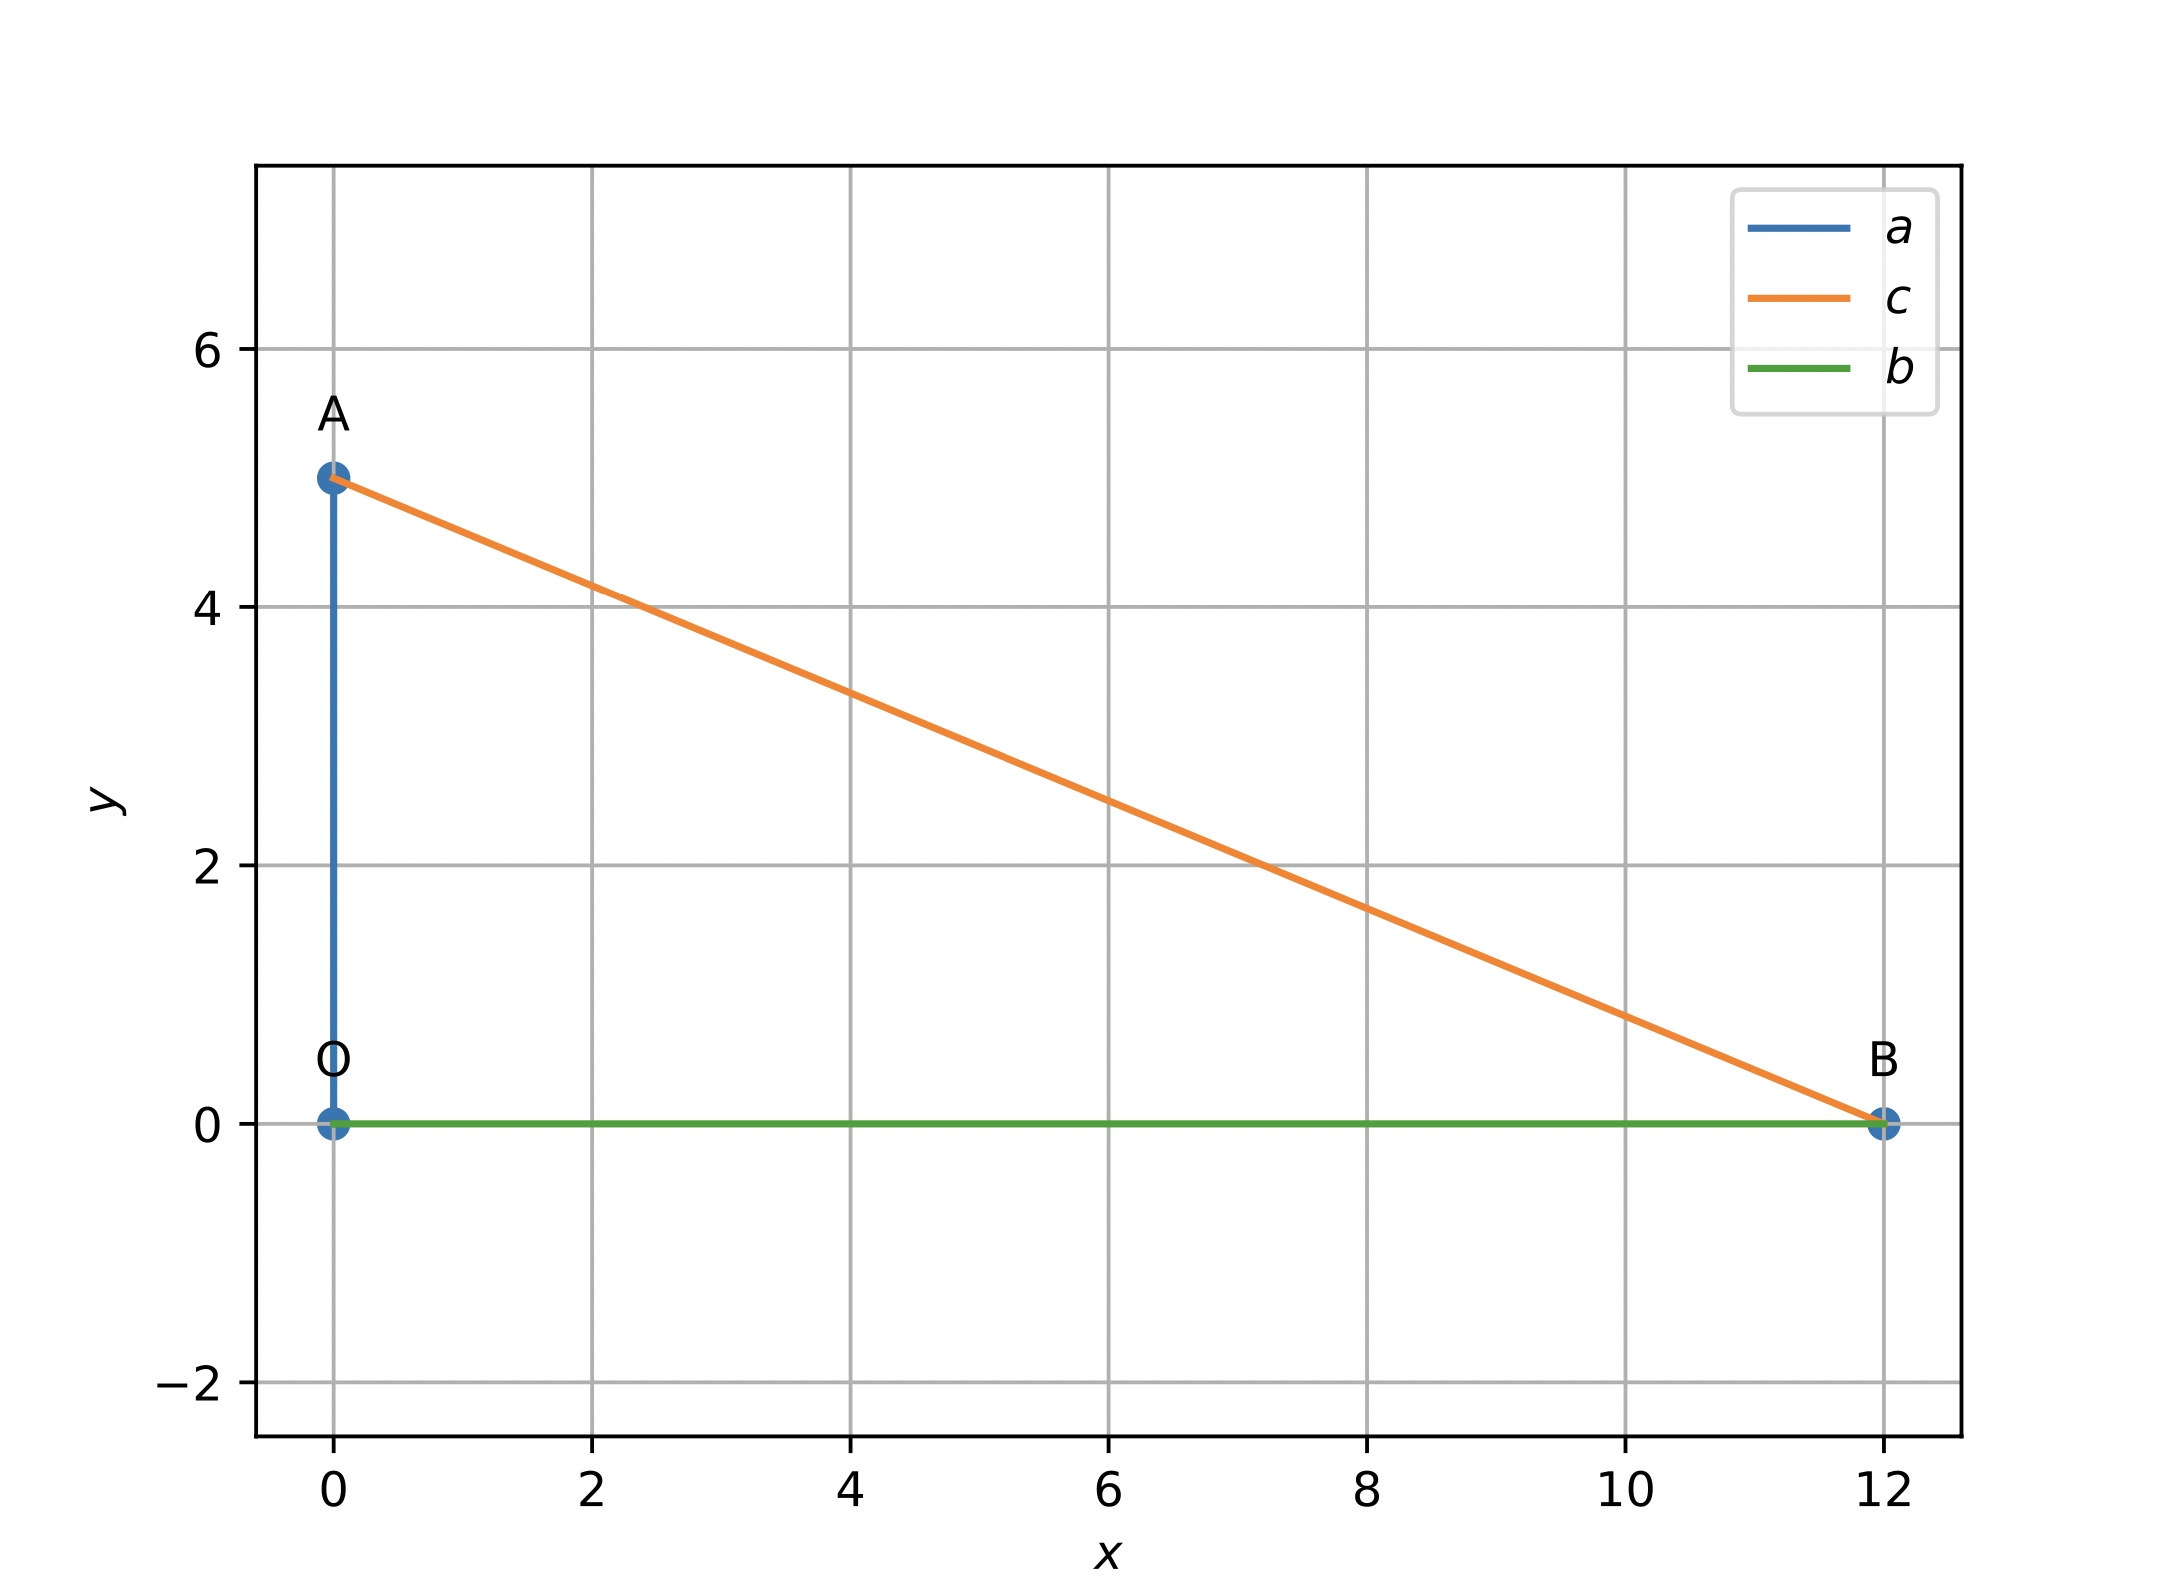
\includegraphics[width=0.5\textwidth]{matrix.jpg}  
 fig 1.2   \vspace{2mm}\\
 \end{center}\vspace{5mm}
 \vspace{2mm}  
\textbf{implementation}
\begin{center}
\setlength{\arrayrulewidth}{0.5mm}
\setlength{\tabcolsep}{5pt}
\renewcommand{\arraystretch}{3}
    \begin{tabular}{|l|c|}
    \hline 
    \textbf{Equation no} & \textbf{Role} \\ \hline
    7 &  Pythagorean Theorem \\ 
    14 & Matrix form of Linear equation  \\
    19 & Results Identity matrix  \\
    21 & Length of $\boldsymbol{c}$\\
    22 & Length of $\boldsymbol{a}$\\
    23 & substituting k=5\\
    \hline
      \end{tabular}
  \end{center} \vspace{2mm}
  
 \vspace{2mm} \textbf{Construction}
\begin{center}
\setlength{\arrayrulewidth}{0.5mm}
\setlength{\tabcolsep}{5pt}
\renewcommand{\arraystretch}{3}
    \begin{tabular}{|l|c|}
    \hline 
    \textbf{vertex} & \textbf{coordinates} \\ \hline
    O & (0,0)  \\ 
    A & (0,5)  \\
    B & (12,0) \\
    \hline
      \end{tabular}
  \end{center}
  
\raggedright  Download the code \\
Github link: \href{https://github.com/chiragshah1244/FWC/blob/main/assignments/assignment_4/code/triangle.py}{Assignment-4}.
  \end{multicols}
\end{document}